The chosen model system of five inhibitors of CHK1 kinase exemplifies different core-hopping transformations (i.e. ring size change, ring opening/closing, ring extension) and R-group modifications \cite{Wang2017}, increasing the complexity compared to the systems previously studied with RE-EDS. Furthermore, the performance can be directly compared to the results obtained with FEP+ and OPLS3 in Ref.~\cite{Wang2017} as well as with QligFEP results in Ref.~\cite{Jespers2019}.

\subsubsection{Parameter Exploration}
The RE-EDS workflow was started by estimating the lower bound for the $s$-distribution. Using the above mentioned undersampling criterion (see Methods section), a lower bound of $s=0.01$ was determined for the protein-ligands complex and $s=0.0056$ for the ligands in water. 

%State Optimizations
A fast transition of the initial maximally contributing end state to the desired maximally contributing end state was observed in the End State Generation. This process was monitored by the maximally contributing end state metric over time.
The transition occurred latest after $1.3$~ns, and the system remained in the biased end state for the rest of the simulation time.
In both water and complex simulations, the desired end state was sampled about $~99\%$ of the simulation time with the exception of L19 in water (Table \ref{SItab:RingCycleOpenin_sampling_fraction_optimizedStates}).
Optimized coordinates were obtained for all five ligands, as verified by comparing the potential-energy distribution from the EDS simulation with the one extracted from a standard MD simulation of the respective ligand (Figure \ref{SIfig:CHK1_RingOpening_soptimization_efficiency}). 
From these same steps, the potential-energy thresholds for the occurrence sampling ($T_{i}^{\text{phys}}$) and undersampling ($T_{i}^{\text{us}}$) were estimated (Table \ref{SItab:RingCycleOpenin_PotentialTresholds}).

\begin{table}[H]
\centering
\caption{Fraction of the simulation time $f_i^{\text{mc}}$ (in \%) that the desired end state was sampled as the maximally contributing state during the EDS simulation to optimize the coordinates for a desired end state.}
\label{SItab:RingCycleOpenin_sampling_fraction_optimizedStates}
\begin{adjustbox}{max width=\textwidth}

\begin{tabular}{ l | c c }
 Ligand & Water  & Complex \\ 
 \hline
     L1 & 99.84 & 99.97 \\ 
     L17 & 99.99 & 99.97\\
     L19 & 36.07 &  99.98\\
     L20 & 99.99 & 100\\
     L21 & 100 & 99.97 \\
\end{tabular}
\end{adjustbox}
\end{table}

To inspect if the optimized state simulations' results sufficiently represent the target states, a comparison between the target state obtained potential-energy distributions in the EDS simulations with MD simulations consisting of only the target state was conducted (Figure \ref{fig:CHK1_set2_stateOptimization_EnergyDistribution}). 


\begin{table}[H]
\centering
\caption{Potential thresholds for occurrence sampling ($T_{i}^{\text{phys}}$) and undersampling ($T_{i}^{\text{us}}$) determined during the parameter exploration (in kJ~mol$^{-1}$).}
\label{SItab:RingCycleOpenin_PotentialTresholds}
\begin{adjustbox}{max width=\textwidth}
\begin{tabular}{ l | c c |c c| }
 Ligand &\multicolumn{2}{c|}{Water} & \multicolumn{2}{c|}{Complex}\\ 
  & \multicolumn{1}{c}{$T^{\text{phys}}$}& \multicolumn{1}{c|}{$T^{\text{us}}$}&  \multicolumn{1}{c}{$T^{\text{phys}}$}& \multicolumn{1}{c|}{$T^{\text{us}}$} \\ 
 \hline
     L1  & -582.96 & -436.05 & -737.37 & -516.41\\ 
     L17 & -572.41 & -419.16 & -717.95 & -492.83\\
     L19 & -579.13 & -415.91 & -738.95 & -483.78\\
     L20 & -636.00 & -492.75 & -759.01 & -549.35\\
     L21 & -656.22 & -488.43 & -805.30 & -539.78\\
\end{tabular}
\end{adjustbox}
\end{table}


%Eoff:
The energy offsets $\vec{E}^R$ were estimated from a short RE-EDS simulation with the PEOE \cite{Sidler2016} scheme and are listed in Table \ref{tab:CHK1_set2_Eoff}.
For $s=1.0$, the energy offsets should ideally be equal to the free energy of the corresponding state (i.e. $\Delta E^R_{ji} = \Delta G_{ji}$) such that the partition function of the reference state is the sum of the partition functions of the end states \cite{Christ2008}. Therefore, the comparison between the relative estimated energy offsets in water and in complex ($\Delta \Delta E^R_{ji} = \Delta E^R_{ji,\text{complex}} - \Delta E^R_{ji,\text{water}}$) and the relative binding free energy $\Delta \Delta G^\text{bind}_{ji}$ can be used to (roughly) assess the quality of the estimated energy offsets. As shown in Figure \ref{fig:CHK1_set2_stateOptimization_EnergyDistribution},
the energy offsets estimated from the SSM simulations are in better agreement with the experimental relative binding free energies than those estimated from the 1SS simulations.
The relative energy offsets $\Delta \Delta E^R_{ji}$ are compared with the experimental relative binding free energies $\Delta \Delta G^\text{bind}_{ji}$ in Figure \ref{SIfig:Eoff_experiment_corr_RingOpening}. 
The RMSE between $\Delta \Delta E^R_{ji}$ obtained with RE-EDS 1SS and $\Delta \Delta G^\text{bind}_{ji}$ is $12.6$~kJ~mol$^{-1}$. Outliers are mainly related to L19.
With the RE-EDS SSM approach, the RMSE was reduced to $7.0$~kJ~mol$^{-1}$. No clear outliers were observed in this case. Thus, the use of the SSM approach is recommended for RE-EDS simulations.

\begin{table}[h]
\caption{Energy offsets $\vec{E^R}$ estimated from a short RE-EDS simulation using the PEOE \cite{Sidler2016} scheme. The errors indicate the standard deviation over the different replicas in undersampling. All energy offsets were calculated relative to ligand L1. The starting coordinates were selected following the 1SS or the SSM approach (see Theory and Methods sections).}
\label{tab:CHK1_set2_Eoff}
\centering
\begin{adjustbox}{max width=\textwidth}
\begin{tabular}{ l | r r | r r }
 Ligand & \multicolumn{2}{c|}{Water}&\multicolumn{2}{c}{Complex}  \\ 
  &RE-EDS 1SS &RE-EDS SSM &RE-EDS 1SS &RE-EDS SSM \\ 
  & [kJ~mol$^{-1}$]& [kJ~mol$^{-1}$]& [kJ~mol$^{-1}$]& [kJ~mol$^{-1}$]\\
 \hline
     L1 & $0.0$ & $0.0$ & $0.0$ & $0.0$ \\ 
     L17 & $11.07 \pm 7.61 $ & $17.81 \pm 0.69 $ & $20.03 \pm 5.04 $ & $18.19 \pm 3.43$ \\
     L19 & $-9.38 \pm 6.85 $ & $ -12.37 \pm 5.23 $ & $-2.09 \pm 1.56 $ & $ 2.4 \pm 1.56$ \\
     L20 & $-53.15 \pm 2.95 $ & $ -56.01 \pm 13.67 $ & $ -58.73 \pm 4.87 $ & $-52.2 \pm 2.6$\\
     L21 & $-76.75 \pm 5.79 $& $-69.15 \pm 3.74 $ & $ -77.29 \pm 3.12 $ & $ -77.9 \pm 3.4$\\
\end{tabular}
\end{adjustbox}
\end{table}

\begin{figure}[h]
\centering
     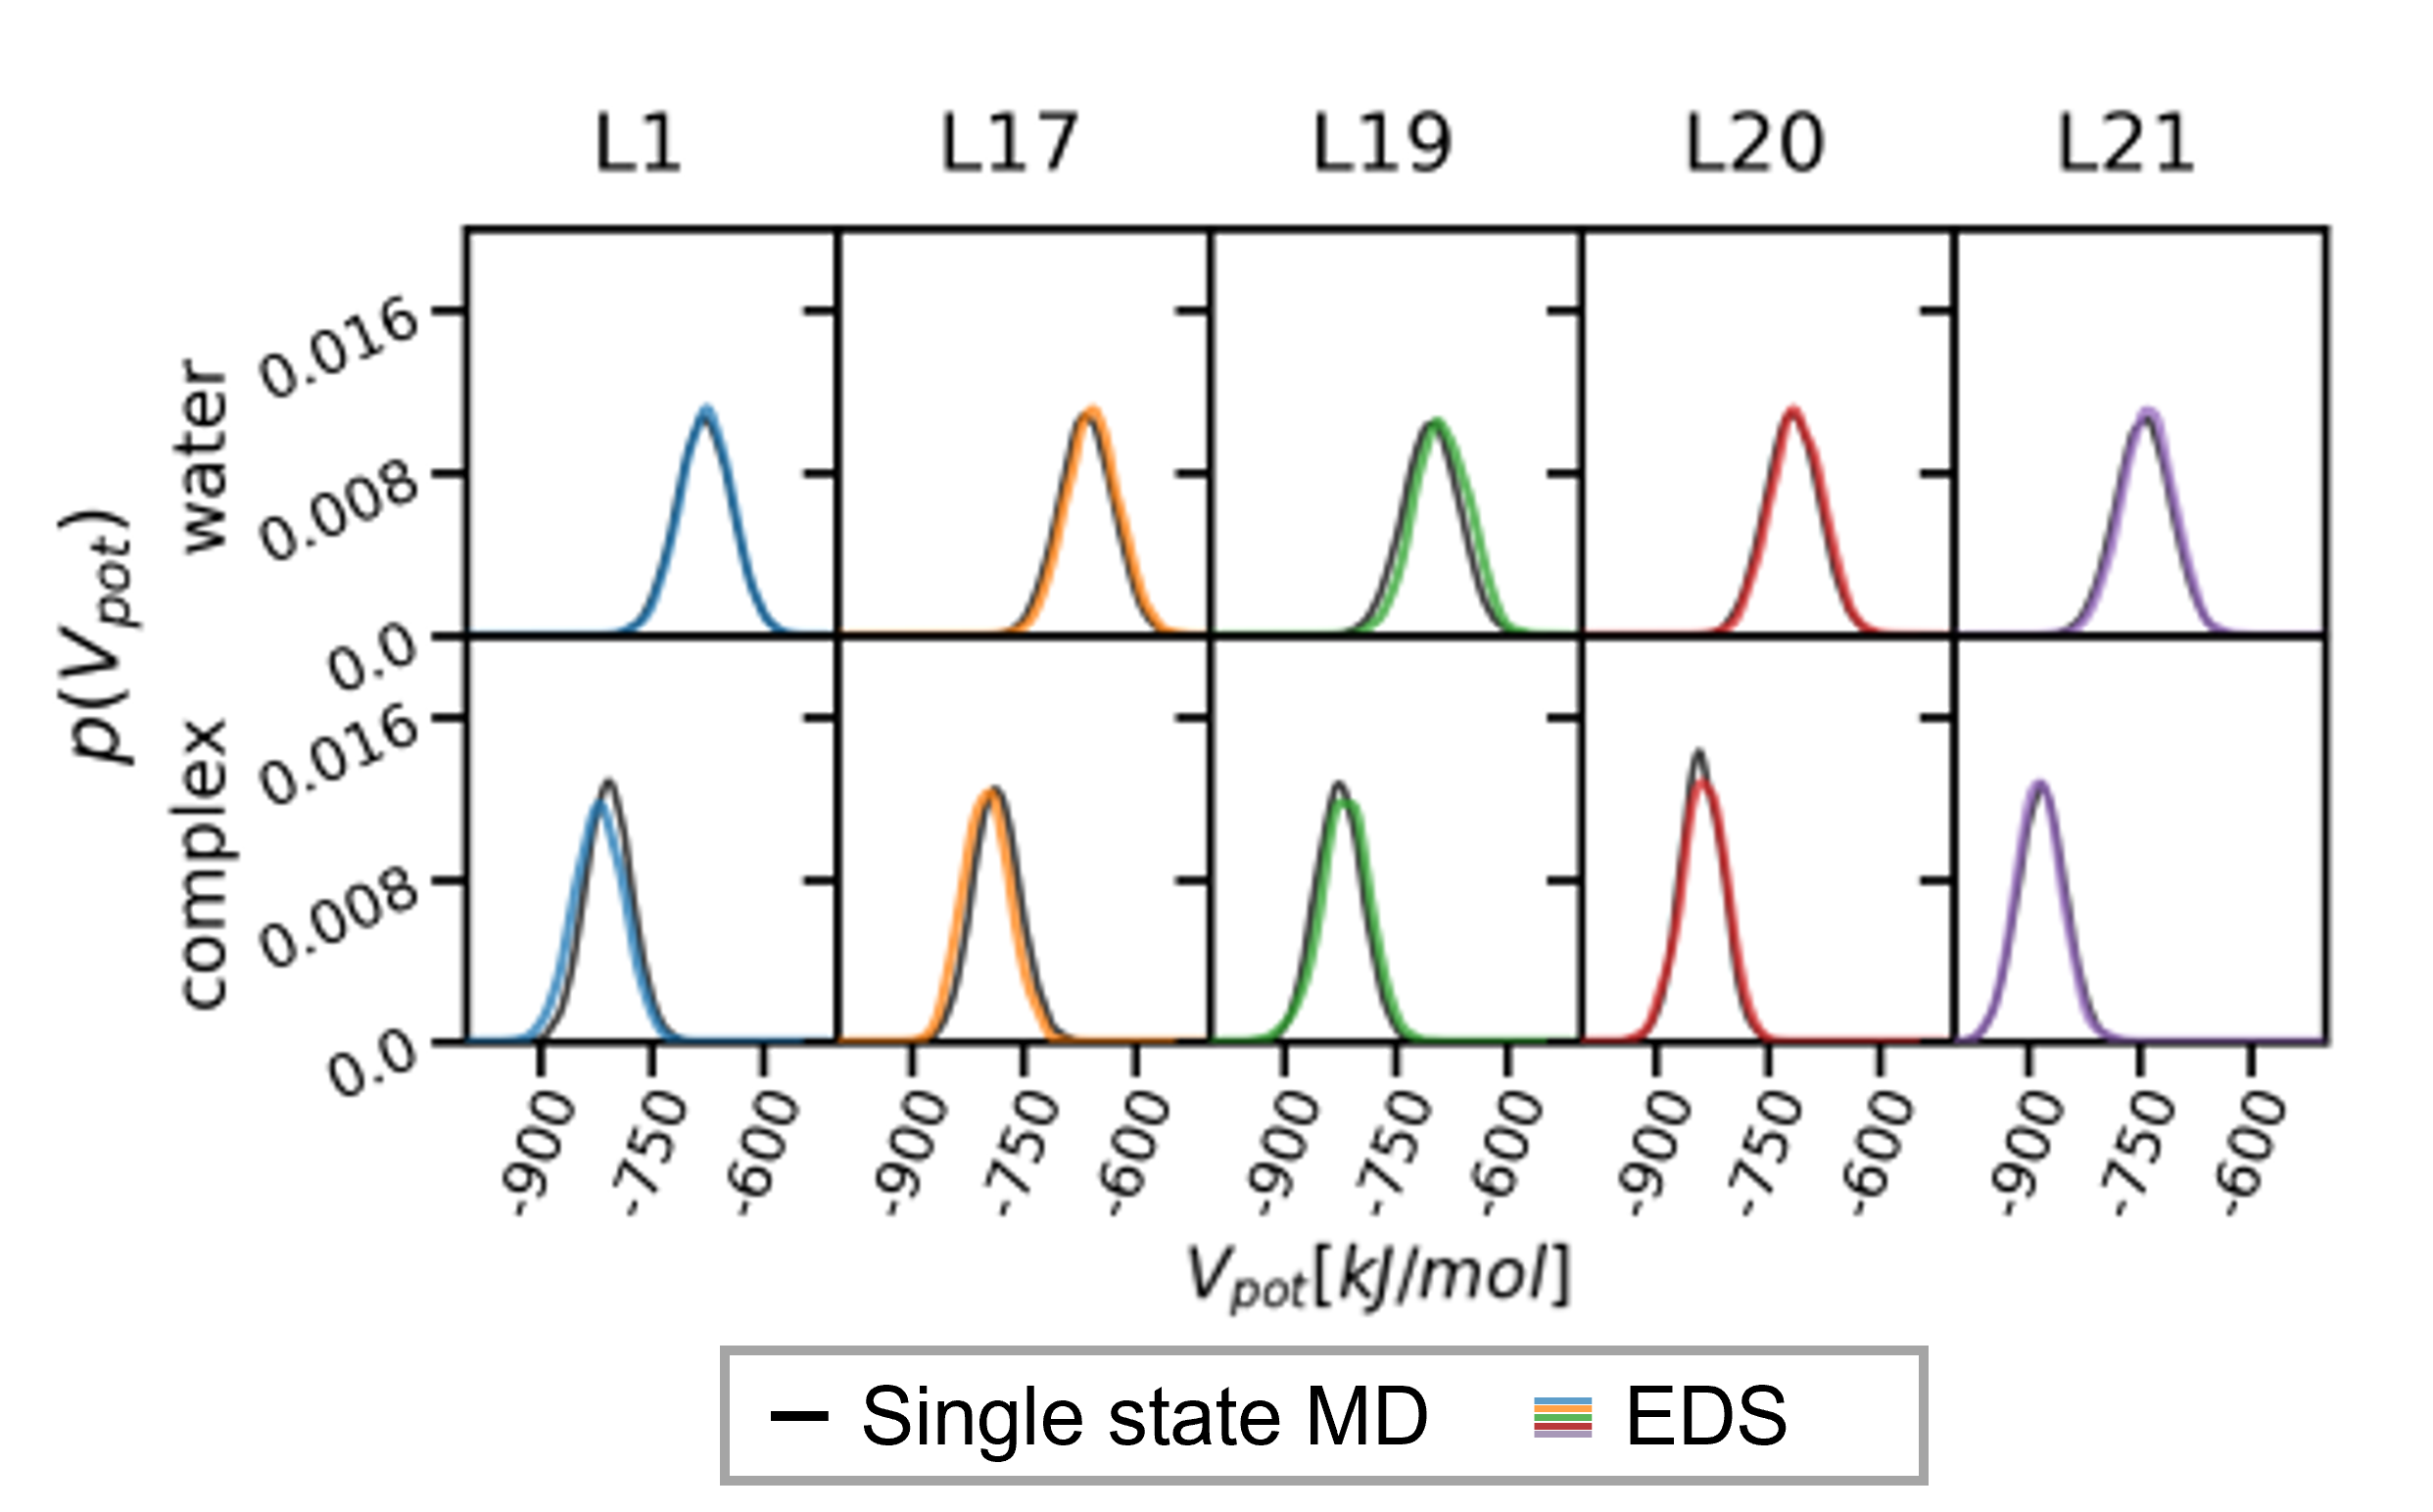
\includegraphics[width=\textwidth]{fig/results/ringOpening/paramExploration/single_state_energy_sampling.png}
    \caption{Comparison of the potential-energy distribution obtained from a standard MD simulation of a given end state (black) and from an EDS simulation with the given end state favoured (colored) from the first step of the RE-EDS workflow.}
     \label{fig:CHK1_set2_stateOptimization_EnergyDistribution}
\end{figure}


\begin{figure}[h]
\centering
  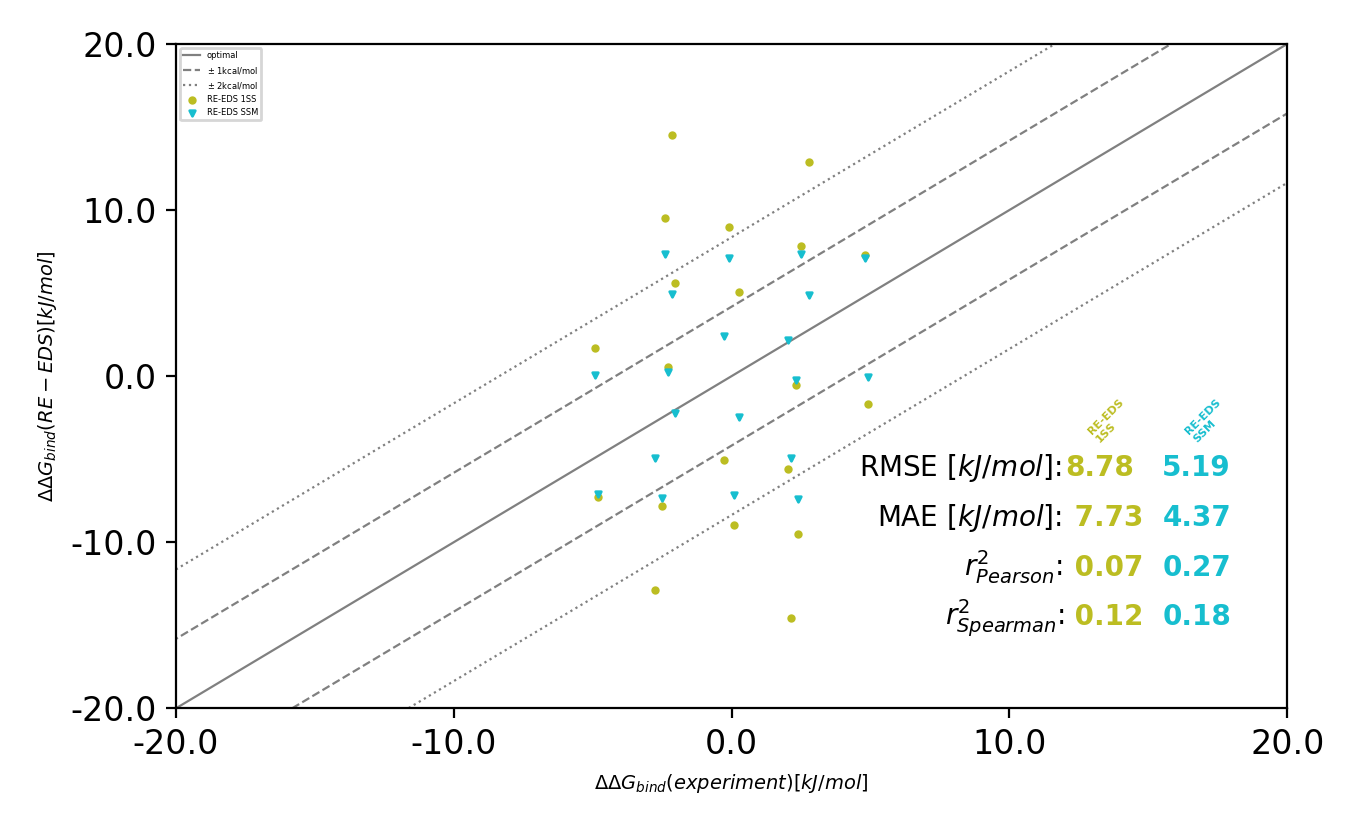
\includegraphics[width=\textwidth]{fig/results/ringOpening/paramOptimization/RingClosure_system_Eoff_final_results.png}
\caption{Comparison of the relative energy offsets $\Delta \Delta E^R_{ji}$ in water and complex with the experimental relative binding free energies $\Delta \Delta G^\text{bind}_{ji}$. The energy offsets were estimated from RE-EDS simulations using the 1SS (green) or SSM (blue) approach to select the starting configurations of the replicas.} \label{SIfig:Eoff_experiment_corr_RingOpening}
\end{figure}

%---------------------------
\FloatBarrier
\clearpage 

\subsection{Parameter Optimization}
%S-Optimization
The optimization of the $s$-distribution was performed with the N-LRTO \cite{Sidler2017} algorithm, thereby minimizing the average round-trip time $\overline{\tau}$ in the replica graph. For the 1SS complex system, four optimization iterations were used. For the other systems, three iterations were used. 

%EoffRB
In the first iteration, the total number of observed round trips was very low or zero for all approaches. In the following iterations, this quantity increased, and the average round-trip time decreased for all simulations (Figure \ref{fig: CHK1_RingOpening_sOptimization}). The number of round trips was generally smaller in the complex than in water due to a more pronounced gap region \cite{Sidler2017}.
Already after the second iteration, the round-trip time was reduced in all approaches. The improvement of the $\overline{\tau}$ over the iterations can also be seen in Figure \ref{SIfig:CHK1_RingOpening_soptimization_efficiency}.

\begin{figure}[h!]
\centering
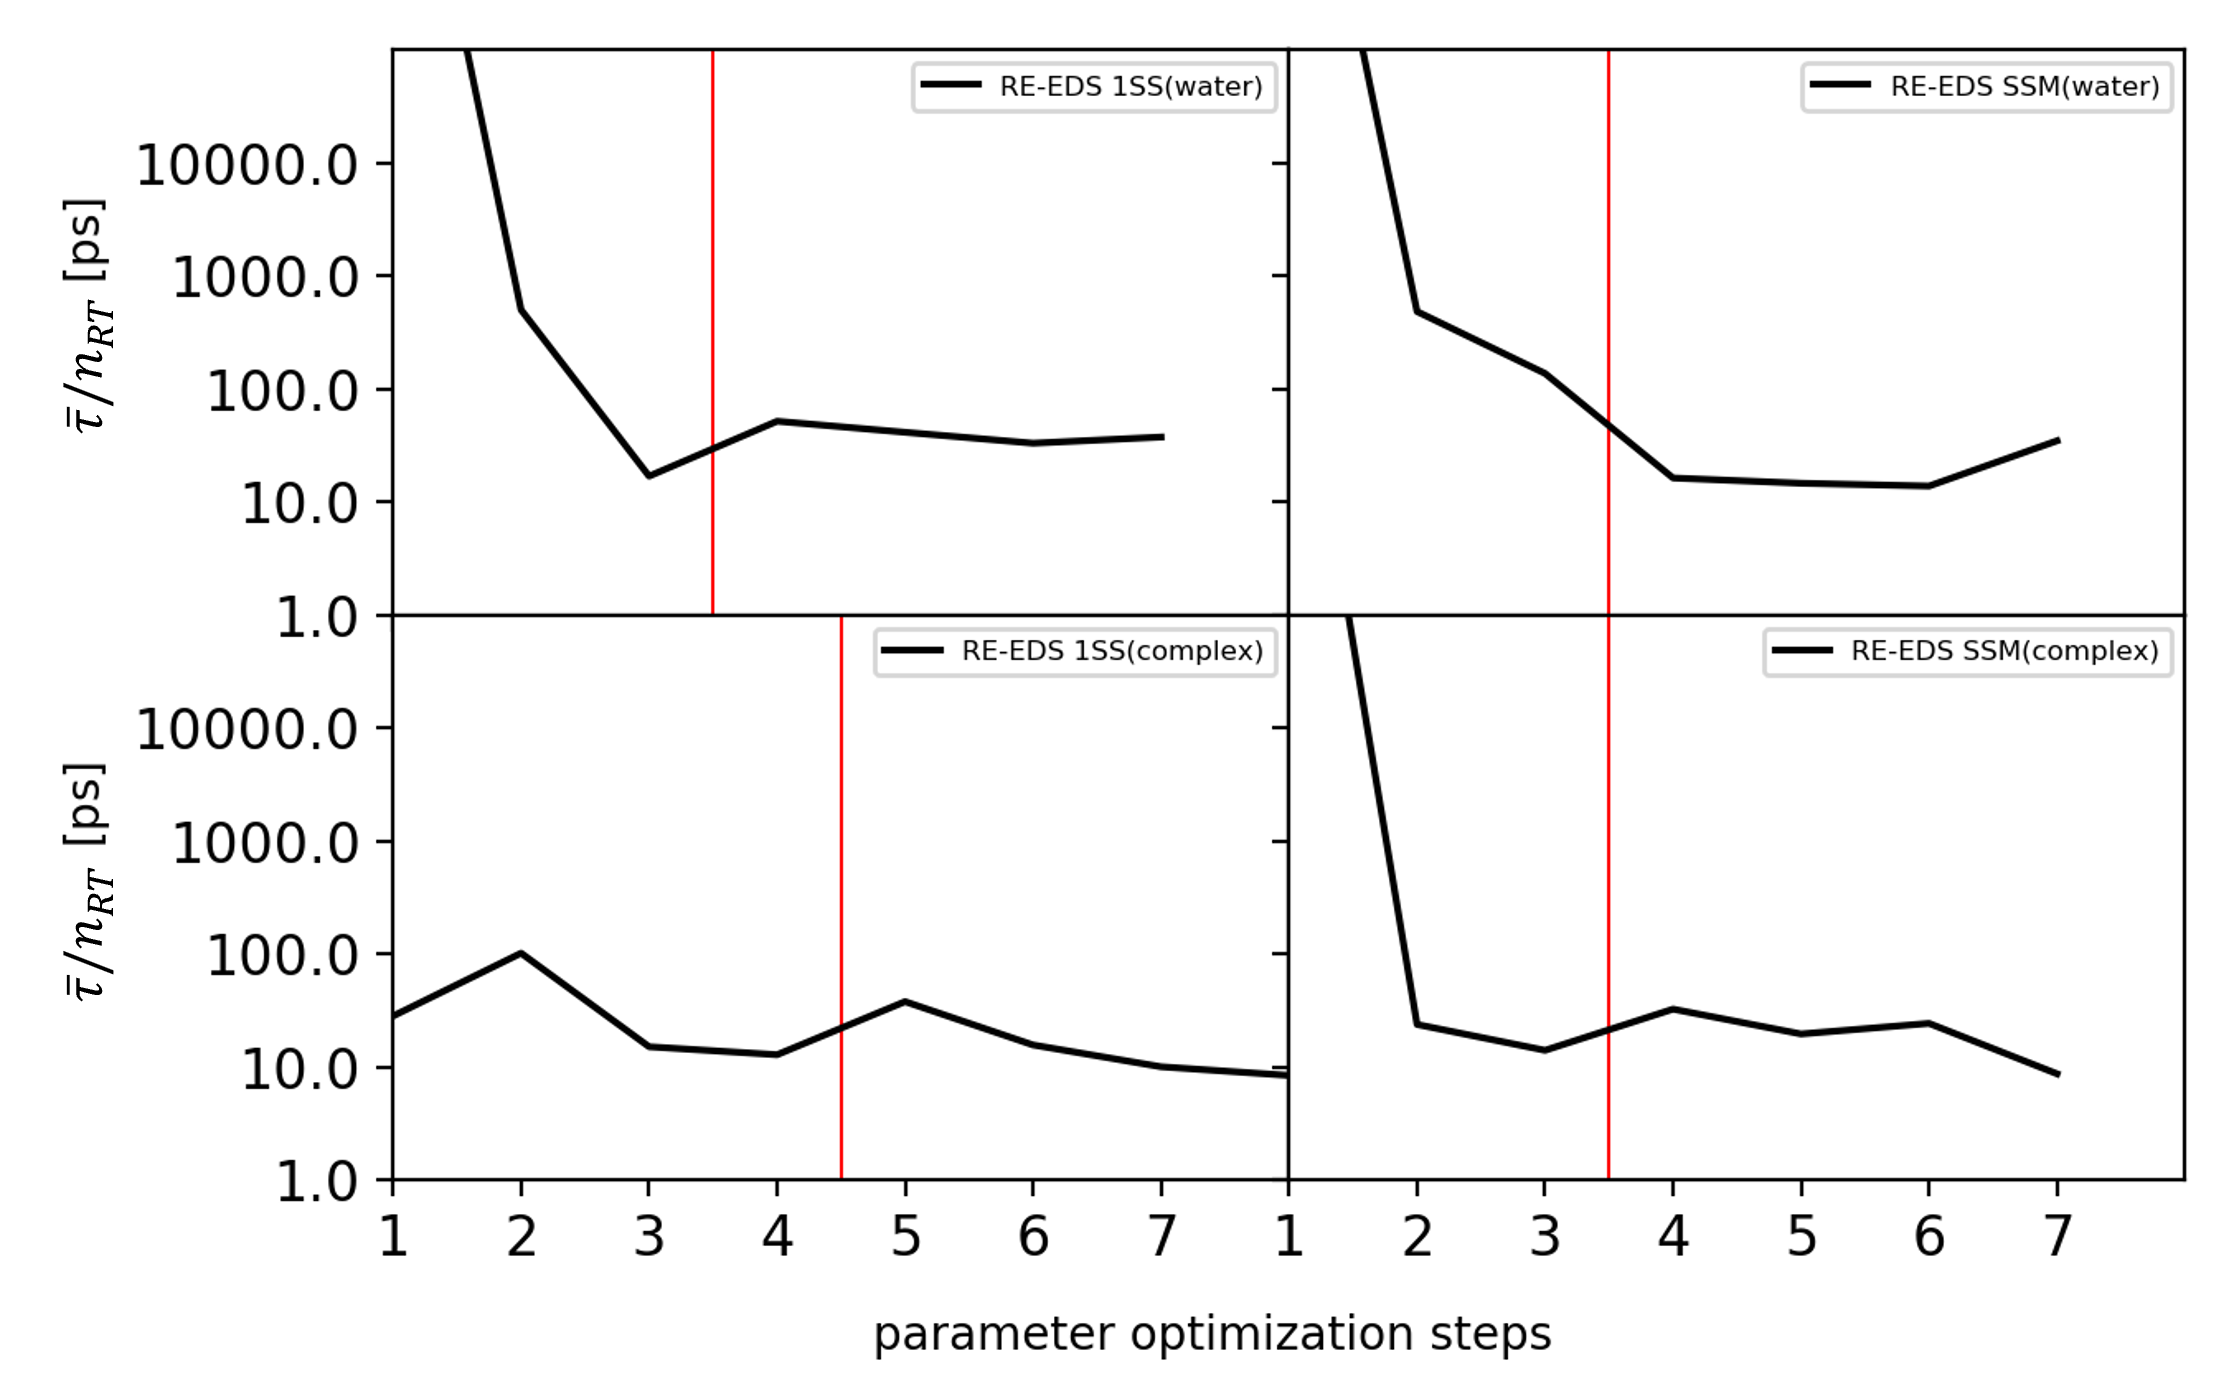
\includegraphics[width=\linewidth]{fig/results/ringOpening/paramOptimization/RingOpening_optimization_RTstat.png}
\caption{Average round-trip time as a function of the optimization steps $i$ ($\overline{\tau}_i$) on a logarithmic scale. The red line indicates the switch from $s$-optimization to energy offset rebalancing.}
\label{SIfig:CHK1_RingOpening_soptimization_efficiency}
\end{figure}

%% s-replica placements
As can be seen in the third row of Figure \ref{fig: CHK1_RingOpening_sOptimization}, the optimization algorithm increases the density of the replicas around $s = 0.041$, where the major gap region lies.

\begin{figure}[h]
\centering
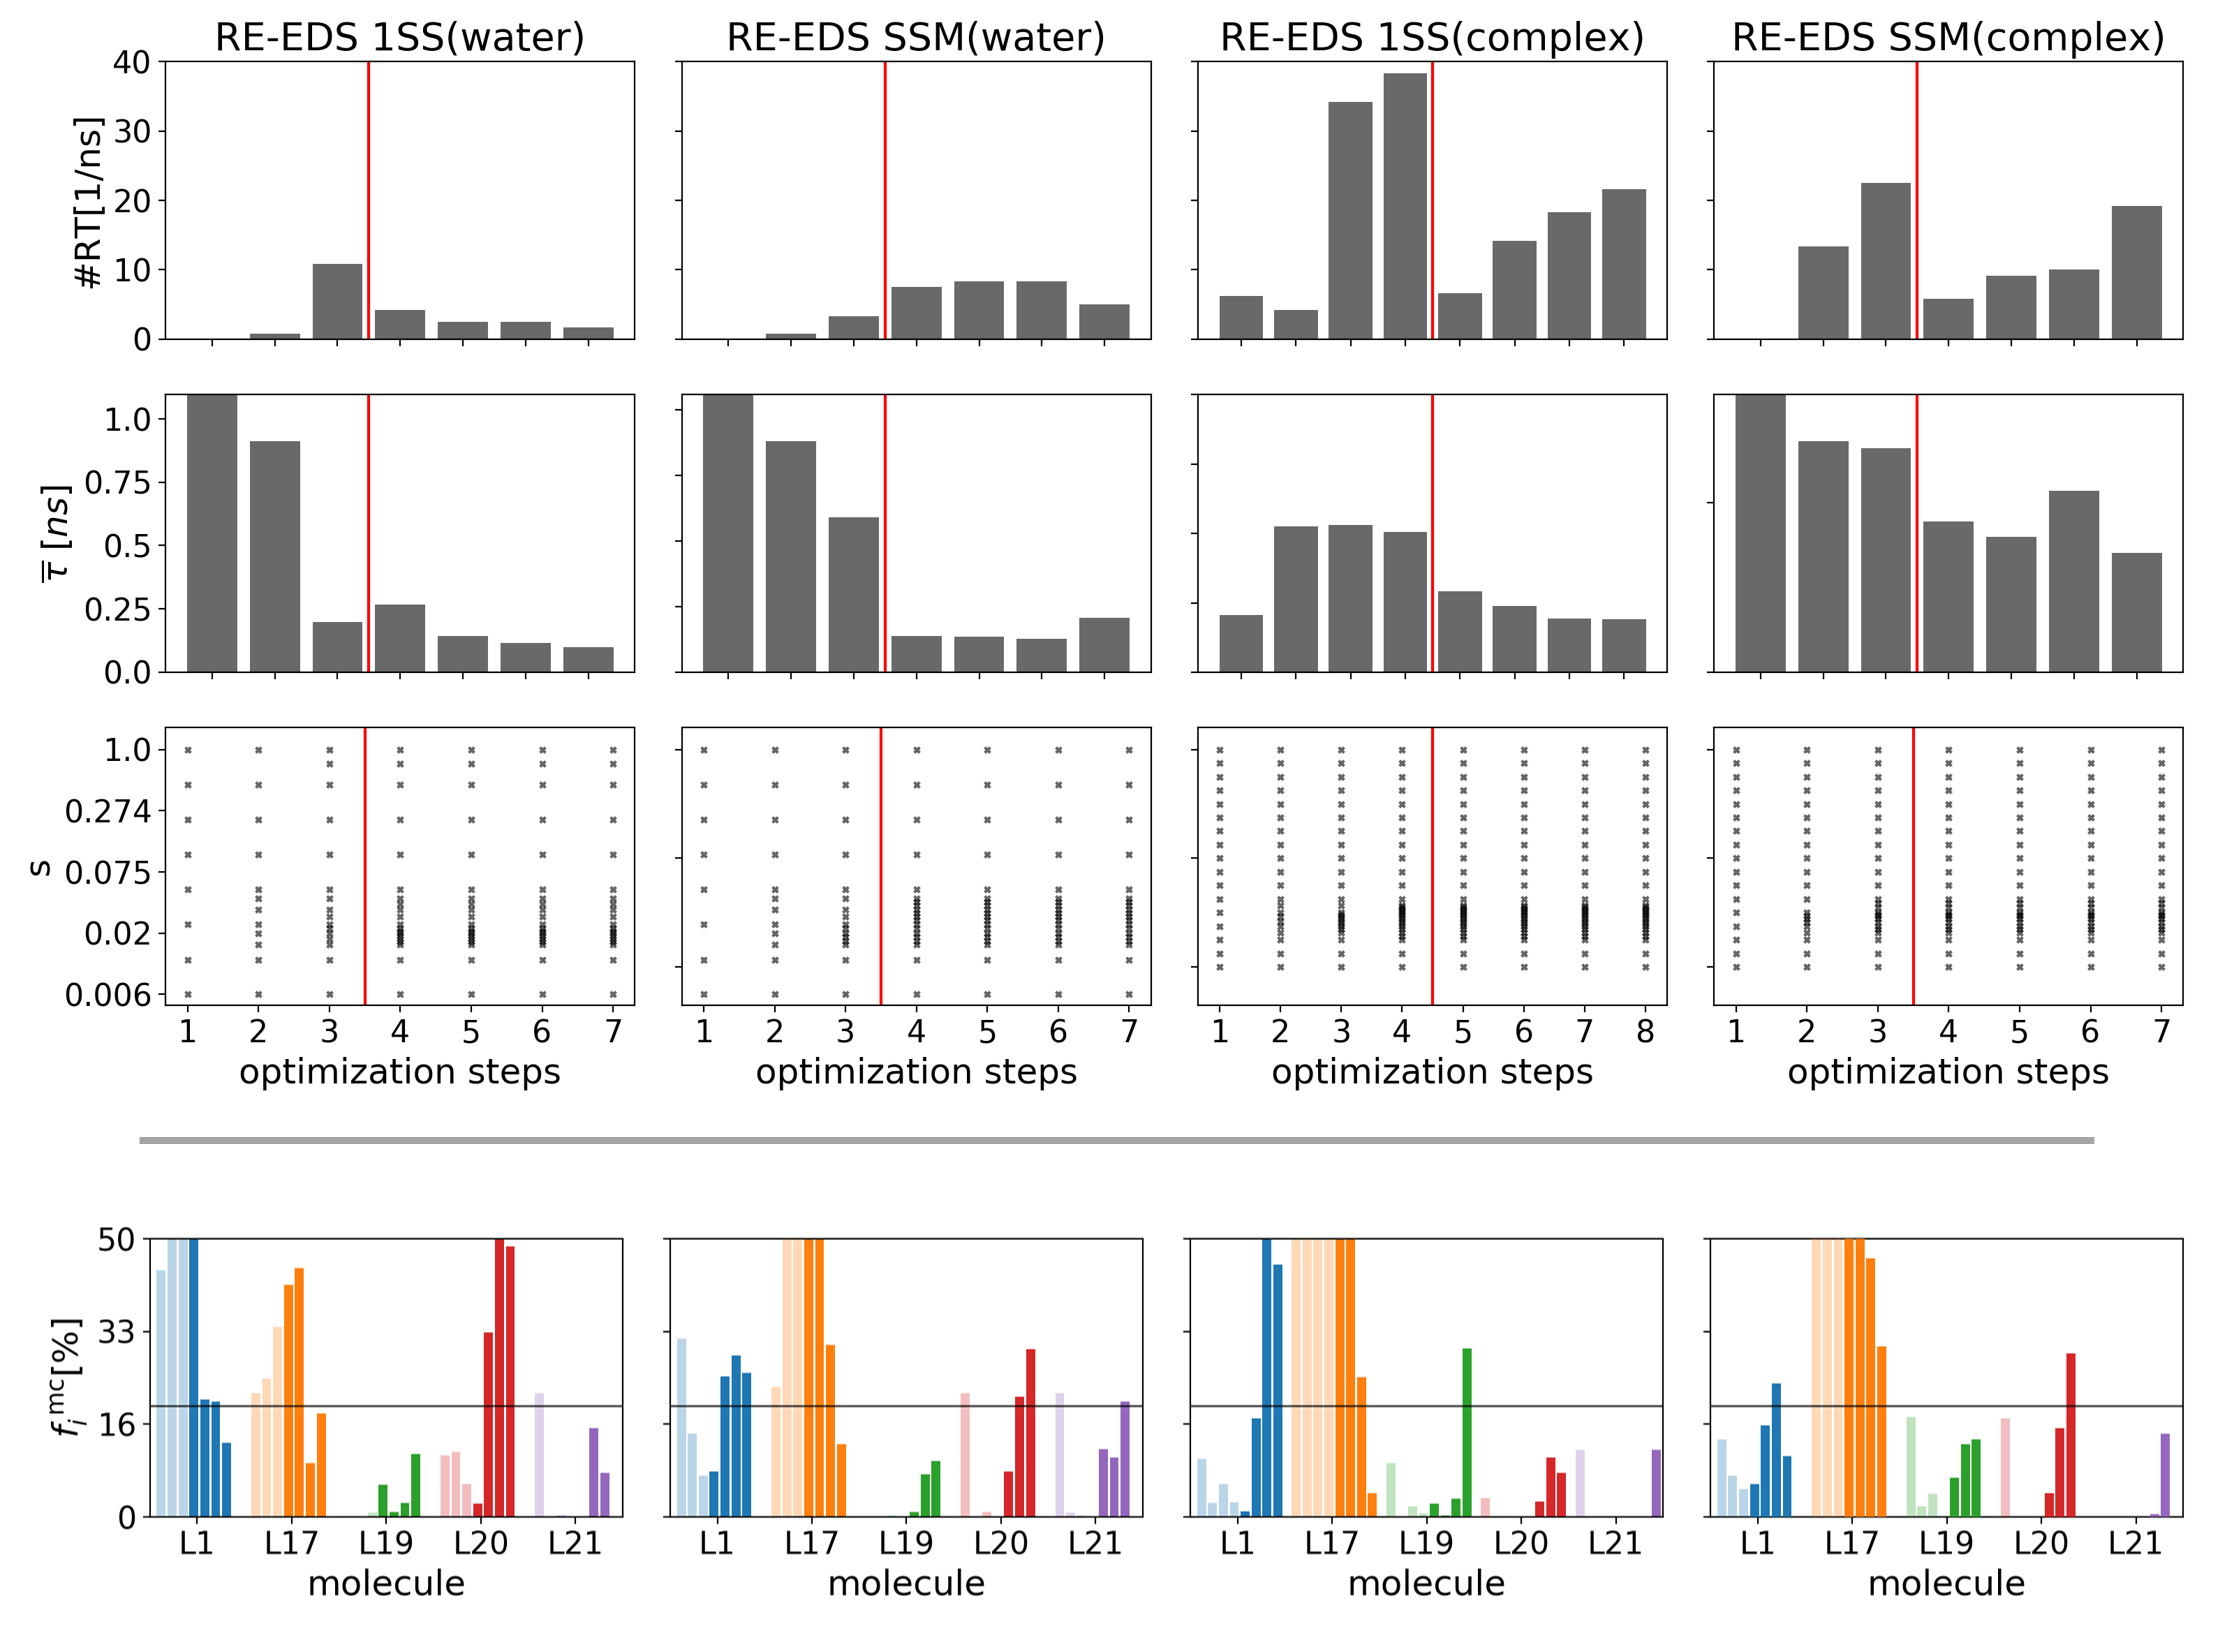
\includegraphics[width=\textwidth]{fig/results/ringOpening/paramOptimization/S-optimization_ringOpening.png}
\caption{Optimization steps of the $s$-distribution with the N-LRTO \cite{Sidler2017} algorithm followed by the energy offset rebalancing scheme (start indicated by the red horizontal line). The measured quality criteria were the number of round trips (1. row), the average round-trip time $\overline{\tau}$ (2. row), the placement of the replicas in $s$-space (3. row), and the sampling fractions of maximally contributing states $f_{i}^{\text{mc}}$ (4. row). The light colored bars of $f_{i}^{\text{mc}}$ indicate $s$-optimization iterations, whereas the fully colored bars indicate energy offset rebalancing steps. }
\label{fig: CHK1_RingOpening_sOptimization}
\end{figure}


%% tau converge - Conclusion
The $s$-optimization was stopped after a sufficiently high number of round trips and low round-trip time was reached. 
This resulted in 20 replicas for the ligands in water after three $s$-optimization iterations.
For the protein-ligands complex, the fourth $s$-optimization iteration was chosen for the 1SS approach, and the third iteration for the SSM approach, resulting in 29 and 25 replicas, respectively. 
The average round-trip time after convergence was $\overline{\tau} = 0.4 \pm 0.2$~ns for all simulations.

After the $s$-optimization, the energy offset rebalancing scheme was applied to improve the state sampling. 

%RT analysis
During the rebalancing steps, no further replicas were added to the $s$-distribution. It is essential for the success of the rebalancing scheme that round trips occur. Therefore, the number of round trips and average round-trip time were monitored. In all systems, the number of round trips and $\overline{\tau}$ remained relatively stable over the four rebalancing steps. For the RE-EDS 1SS approach in water, the number of round trips slightly decreased but never dropped to zero.

%% states sampling
Across the optimization steps, also the sampling of the end states as maximally contributing states at $s=1.0$ was monitored.
During the $s$-optimization, some end states ``vanish'' and are no longer sampled as maximal contributing states. This leakage effect can occur when the initially estimated $E^{\text{R}}$ are not exactly optimal \cite{Sidler2016}. 
With energy offset rebalancing, the sampling of each end state can be recovered, and the sampling distribution approaches the ideal case.
%After the s-optimization the MAE($P^{\text{maxContrib}}$) was for all approaches approximately at $25\%$, with the exception of the 1SS water system, here it was $20\%$. 
After rebalancing, all end states showed a $f_i^{\text{mc}} > 0$ and the mean absolute deviation of the sampling distribution from ideal decreased from $20-25\%$ to approximately $7-12\%$ (Figure \ref{SIfig:CHK1_RingOpening_optimization_fractOptSampMAE}). 
 


\begin{figure}[h]
\centering
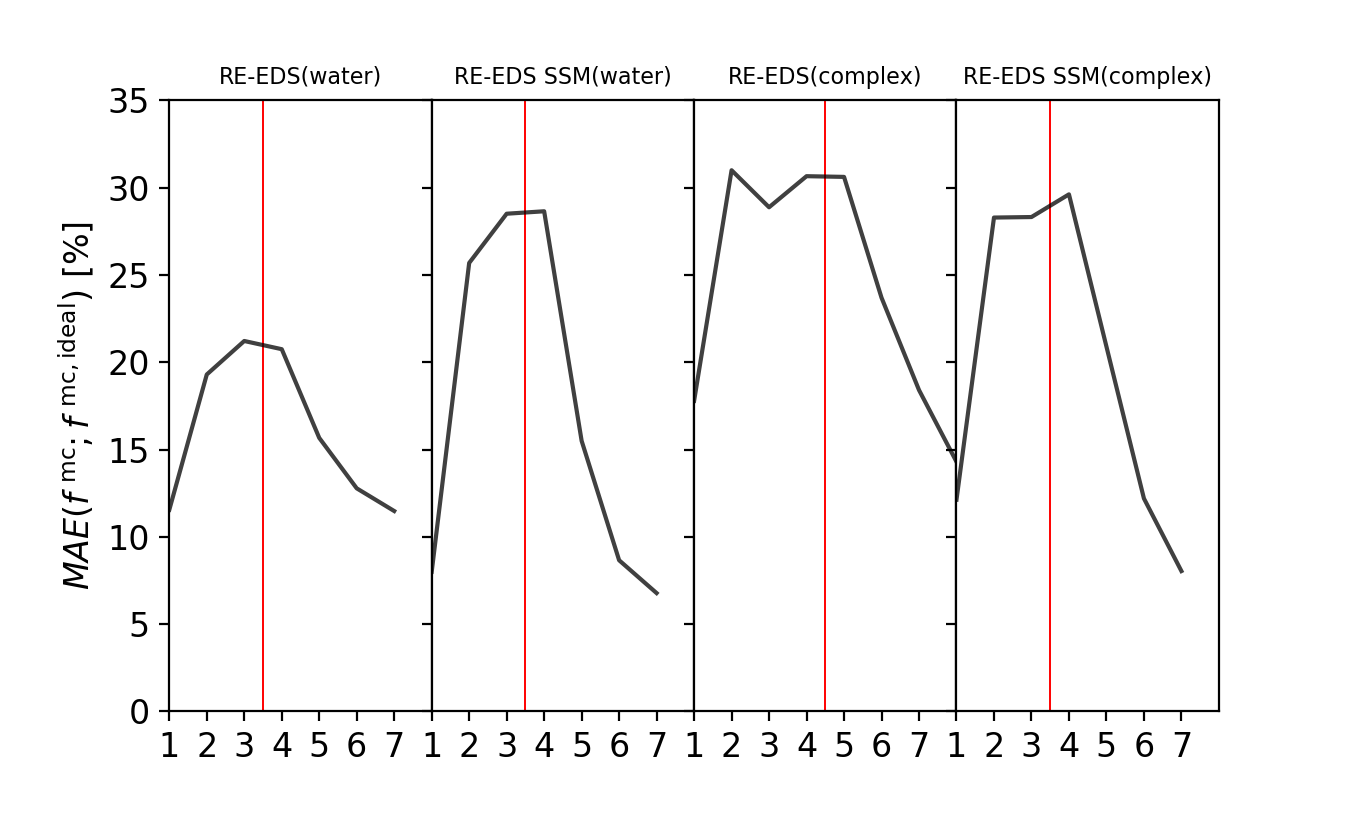
\includegraphics[width=\linewidth]{fig/results/ringOpening/paramOptimization/RingOpening_optimization_fractOptSampMAE.png}
\caption{Mean absolute deviation (MAE, in percentage) of the observed state sampling $f_i^{\text{mc}}$ from the ideal equal distribution $f_i^{\text{mc,ideal}}$ during the short optimization simulations. The red line indicates the switch from $s$-optimization to energy offset rebalancing.}
\label{SIfig:CHK1_RingOpening_optimization_fractOptSampMAE}
\end{figure}

%---------------------------
\FloatBarrier
\clearpage

\subsection{Free-Energy Calculation}
After successfully optimizing the RE-EDS parameters, the production runs were performed for $3.5$~ns. 


%%Sampling++
Both in water and in complex, the potential-energy distributions of the end states generally match well the corresponding distributions from the standard MD simulations of the single end states (Figure \ref{fig:RingOpening_sampling_comparison}). Only in the complex 1SS approach, a deviation can be seen for L17, with a slight shift to higher potential energies. This is due to insufficient sampling of L17 in this case (see below). 
%
The analysis of the maximally contributing end states at $s=1.0$ shows that in water all end states were sampled close to the ideal equal distribution (Figure \ref{SIfig:CHK1_RingOpening_soptimization_final_Sampling_s1}). 
\begin{figure}[H]
\centering
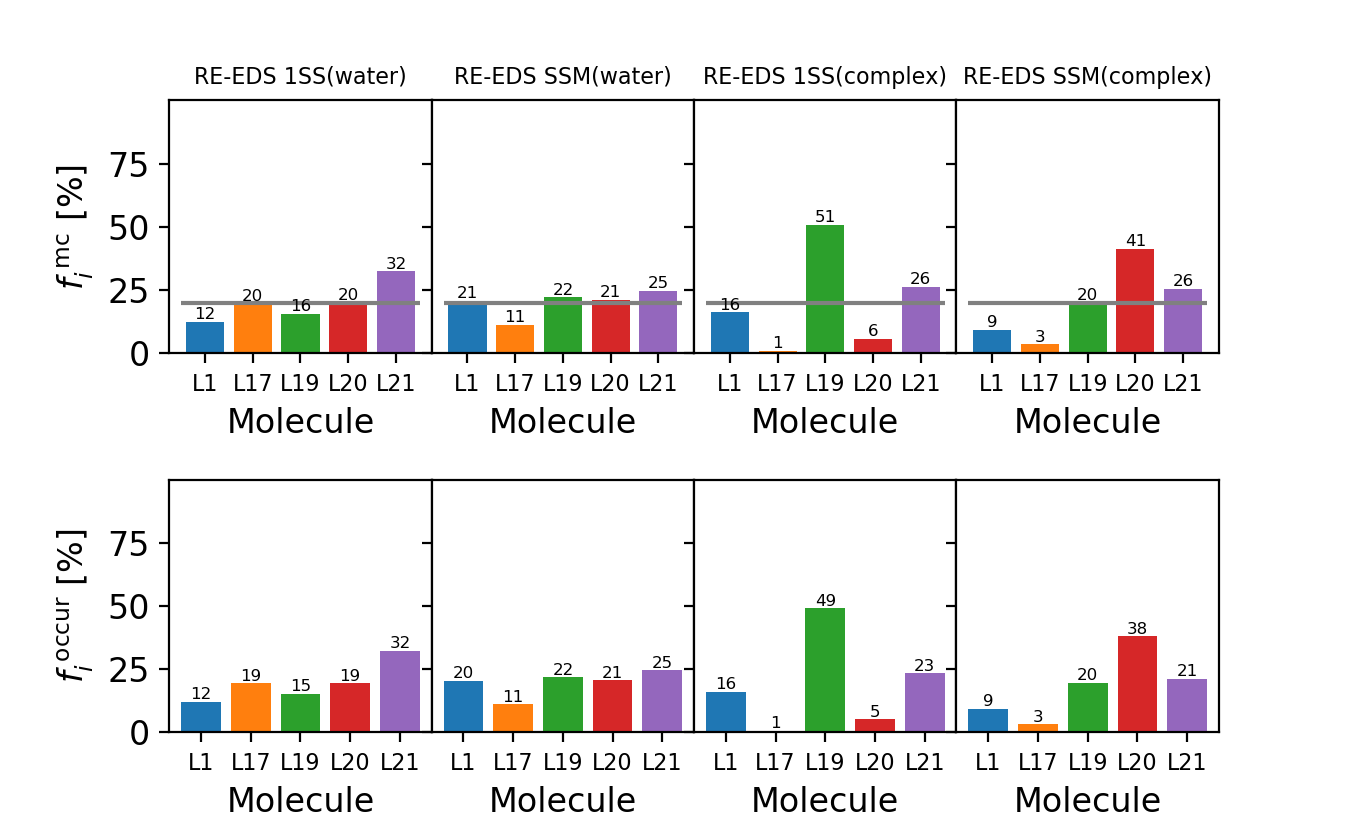
\includegraphics[width=\textwidth]{fig/results/ringOpening/FE/Reeds_RingOpening_production_sampling_s1.png}
\caption{Sampling of the end states in the final production run at replica $s=1.0$. Sampling was assessed by monitoring the maximally contributing end state (top panels) and by counting all end states a potential energy below $T_{i}^{phys}$ (see Table \ref{SItab:RingCycleOpenin_PotentialTresholds}) (bottom panels). Ideally, the sampling fraction as maximally contributing end state should be 1/$N$ (Eq. (8) in the main text) for all end states, indicated as a black horizontal line.}
\label{SIfig:CHK1_RingOpening_soptimization_final_Sampling_s1}
\end{figure}


In the simulation of the protein-ligands complex, there are still differences in sampling. Especially with the 1SS approach, L19 is generally sampled too much, while L17 is not sampled enough. The situation is improved with the SSM approach.
Comparing $f_i^{\text{occur}}$ and $f_i^{\text{mc}}$ in Figure \ref{SIfig:CHK1_RingOpening_soptimization_final_Sampling_s1} indicates that the end states in the CHK1 system are clearly separated (i.e. no phase-space overlap).

\begin{figure}[h]
    \centering
    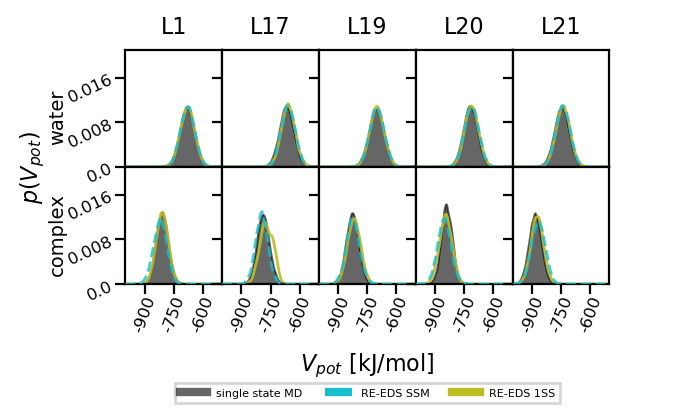
\includegraphics[width=\columnwidth]{fig/results/ringOpening/FE/RingClosure_system_final_sampling.png}
    \caption{Comparison of the Boltzmann reweighted potential-energy distributions obtained from standard MD simulations of a given end state (black) and from the RE-EDS production runs of the 1SS (green) and SSM (turquoise, dashed) approaches.}
    \label{fig:RingOpening_sampling_comparison}
\end{figure}

%%Accuracy
From the replica at $s=1.0$, the free-energy differences were calculated using Eq.~(\ref{EQ: Free Energy calculation via reference state}) and the resulting $\Delta \Delta G^\text{bind}_{ji}$ were compared with the experimental results taken from Ref.~\cite{Huang2012}. The results are shown graphically in Figure \ref{fig:CHK1_set2_FreeEnergyCalculation} and numerically in Table \ref{tab: RE-EDS_FE_RingCycleOpening_ddF}. The individual free-energy differences are given in Table \ref{SItab: RE-EDS_FE_RingCycleOpening_dFs}.
The RMSE with RE-EDS 1SS is $4.4$~kJ~mol$^{-1}$ and the MAE is $3.9\pm2.8$~kJ~mol$^{-1}$. 

\begin{table}[H]
\caption{Free-energy differences in water and in complex calculated from the production run of 3.5~ns of length with the RE-EDS 1SS and RE-EDS SSM approaches.}
\label{SItab: RE-EDS_FE_RingCycleOpening_dFs}
\begin{center}
\begin{adjustbox}{max width=\textwidth}
\begin{tabular}{ c c |c c |c c}
  \multicolumn{2}{c|}{Ligand} & \multicolumn{2}{c|}{RE-EDS 1SS} &\multicolumn{2}{c}{RE-EDS SSM}\\ 
  J & I  & water [kJ~mol$^{-1}$] & complex [kJ~mol$^{-1}$]  & water [kJ~mol$^{-1}$] & complex [kJ~mol$^{-1}$] \\
  \hline
        L17 &         L1 &       11.9 $\pm$ 0.0&        17.0 $\pm$ 0.8&   12.4 $\pm$ 0.5&   9.4 $\pm$ 1.9\\
        L19 &         L1 &        2.7 $\pm$ 0.0&        5.7 $\pm$ 1.0&     3.1 $\pm$ 0.0&   8.0 $\pm$ 0.0\\
        L20 &         L1 &      -47.8 $\pm$ 0.0&      -47.6 $\pm$ 0.9& -47.7 $\pm$ 0.0&  -48.1 $\pm$ 0.0\\
        L21 &         L1 &      -61.7 $\pm$ 0.06&     -63.1 $\pm$ 0.8& -61.7 $\pm$ 0.0&  -64.8 $\pm$ 0.0\\
        L19 &         L17 &      -9.2 $\pm$ 0.0&      -11.3 $\pm$ 0.6&  -9.3 $\pm$ 0.5&   -1.4 $\pm$ 1.9\\
        L20 &         L17 &     -59.6 $\pm$ 0.0&      -64.5 $\pm$ 0.1& -60.1 $\pm$ 0.5&  -57.6 $\pm$ 1.9\\
        L21 &         L17 &     -73.6 $\pm$ 0.0&      -80.1 $\pm$ 0.1& -74.1 $\pm$ 0.5&  -74.3 $\pm$ 1.9\\
        L20 &         L19 &     -50.5 $\pm$ 0.0&      -53.2 $\pm$ 0.6& -50.7 $\pm$ 0.0&  -56.2 $\pm$ 0.0\\
        L21 &         L19 &     -64.4 $\pm$ 0.0&      -68.8 $\pm$ 0.6& -64.7 $\pm$ 0.0&  -72.9 $\pm$ 0.0\\
        L21 &         L20 &     -13.9 $\pm$ 0.0&      -15.5 $\pm$ 0.2& -14.0 $\pm$ 0.08& -16.7 $\pm$ 0.0 \\
\end{tabular}
\end{adjustbox}
\end{center}
\end{table}

The main deviations stem from ligand L17 in the RE-EDS 1SS approach, which can be explained by the insufficient sampling of L17 in the complex (see Figure \ref{fig:RingOpening_sampling_comparison} and Figure \ref{SIfig:CHK1_RingOpening_soptimization_final_Sampling_s1}).

The performance was substantially improved using the SSM approach with RE-EDS, giving an RMSE of $3.3$~kJ~mol$^{-1}$ and an MAE of $2.8 \pm 1.7$~kJ~mol$^{-1}$. 
Only two values (L21-L11) and (L21-L19) deviate more than $4.184$~kJ~mol$^{-1}$ (i.e. $1$~kcal~mol$^{-1}$) from experiment.
The Spearman correlation coefficient for RE-EDS 1SS is $r_{\text{Spearman}}=0.01$ and for RE-EDS SSM $r_{\text{Spearman}}=0.69$.

%%Performance:
Next, we assessed the convergence of the $\Delta G_{ji}$ values as a function of simulation time (Figure \ref{SIfig:CHK1_RingOpening_dF_convergence}).
\begin{figure}[h]
\centering
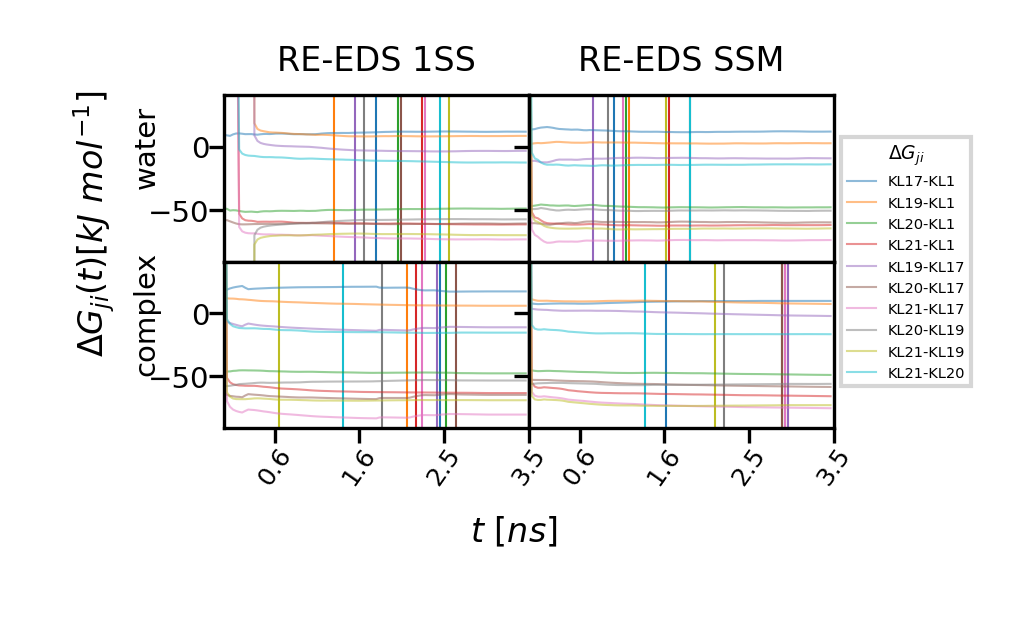
\includegraphics[width=\textwidth]{fig/results/ringOpening/FE/dF_RingOpening_Convergence.png}
\caption{Convergence analysis of the RE-EDS production runs (total 3.5~ns): The free-energy results are plotted as a function of the simulation time. The vertical lines indicate when a particular $\Delta G_{ji}$ value was found to be converged (deviation below 1~kJ~mol$^{-1}$).}
\label{SIfig:CHK1_RingOpening_dF_convergence}
\end{figure}

For the RE-EDS 1SS approach, all free-energy differences appeared converged after $2.5$~ns in water and after $2.7$~ns in the complex. For the RE-EDS SSM approach, convergence was observed after $2.5$~ns in water and after $2.9$~ns in the complex.

\begin{figure}[h]
    \centering
    \begin{subfigure}{0.85\columnwidth}
        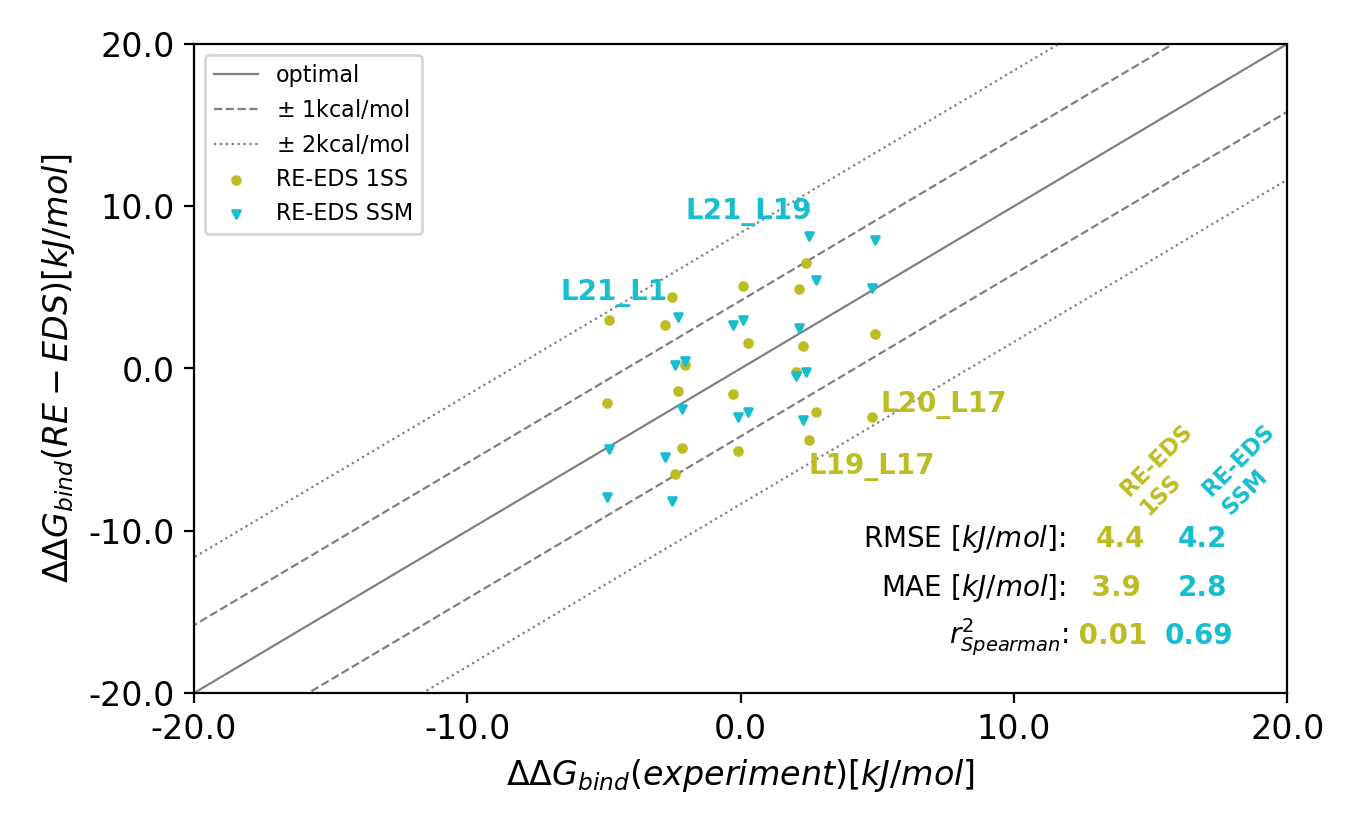
\includegraphics[width=\textwidth]{fig/results/ringOpening/FE/RingClosure_system_final_results_4ns_comparison.png}
        \end{subfigure}
    \begin{subfigure}{0.85\columnwidth}
        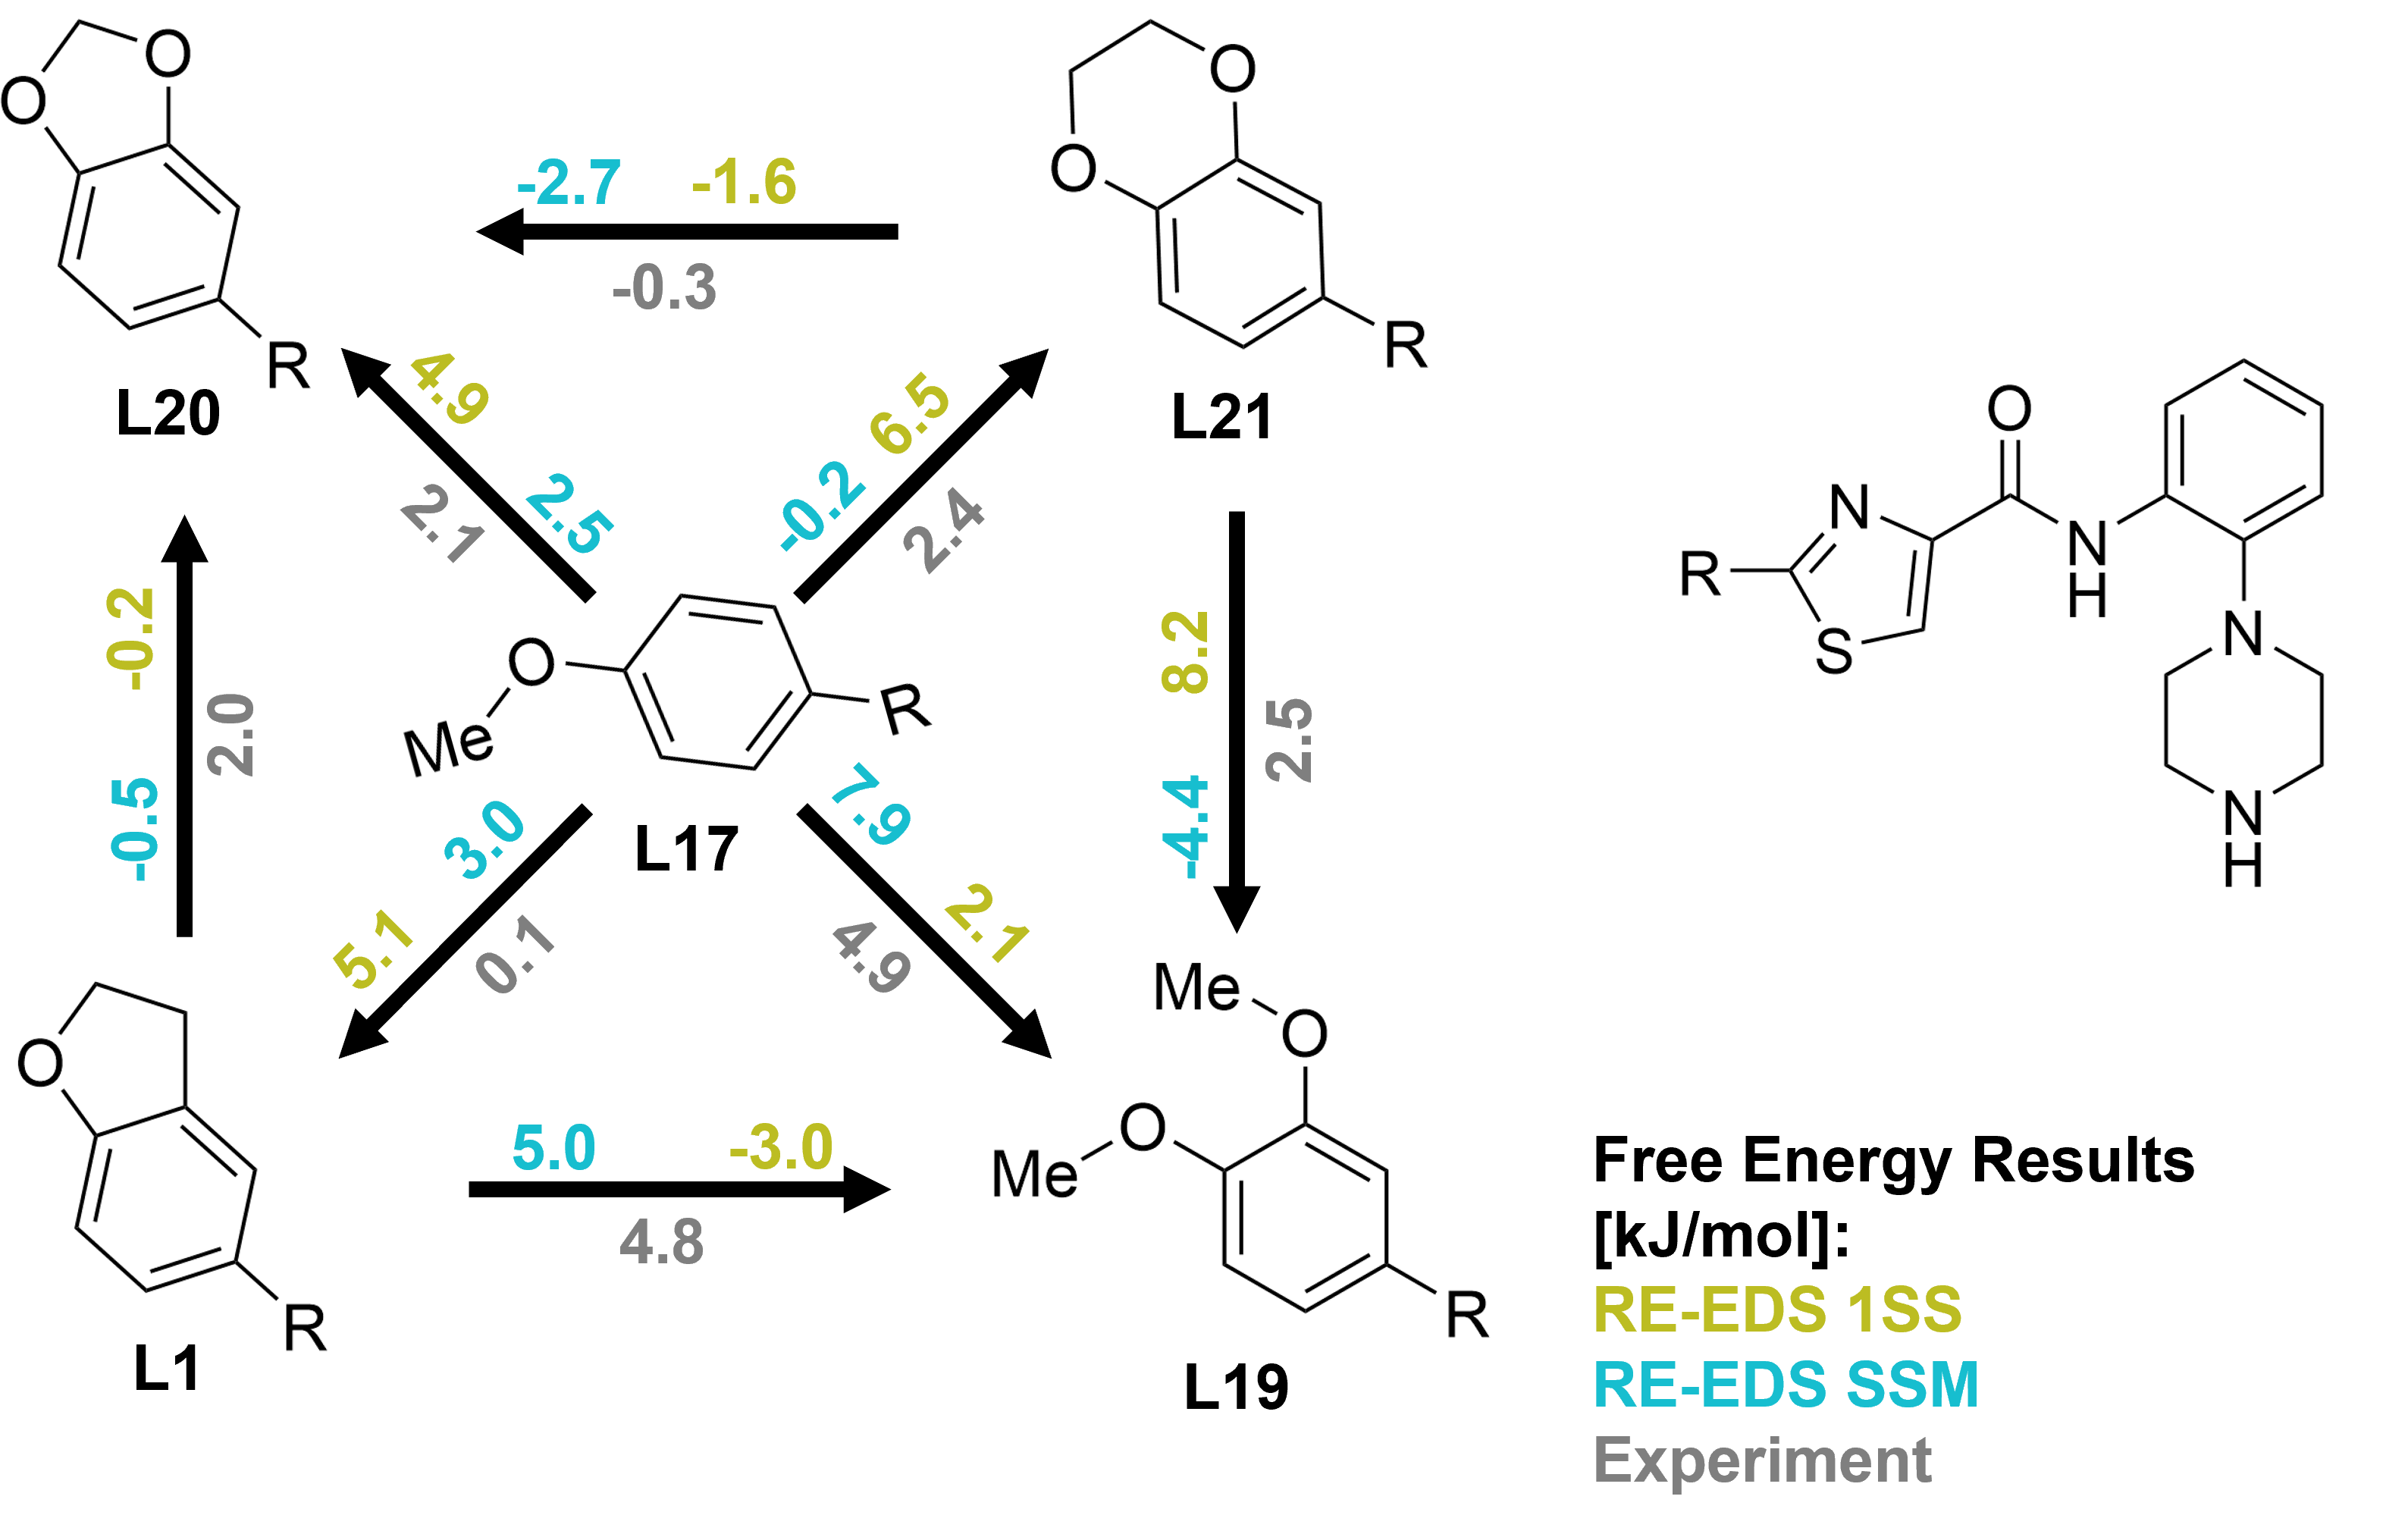
\includegraphics[width=\textwidth]{fig/results/ringOpening/FE/ddG_bind_paper_comparison_reeds_only_4nsSimulation.png}
        \end{subfigure}
    \caption{Free-energy differences estimated from the production run of $3.5$~ns length. (Top): Comparison between the experimental and calculated $\Delta \Delta G^\text{bind}_{ji}$ using RE-EDS 1SS and RE-EDS SSM. The results were calculated with all possible pairwise transformations (forward and backward). (Bottom): Graphical representation of the $\Delta \Delta G^\text{bind}_{ji}$ results with structures, inspired by the one in Ref.~\cite{Wang2017}.}
    \label{fig:CHK1_set2_FreeEnergyCalculation}
\end{figure}

%Comparison results with Schroedinger & Jespers
By applying the RE-EDS methodology to the same system of five CHK1 inhibitors as studied by Wang \textit{et. al.} \cite{Wang2017} and later on also Jespers \textit{et al.} \cite{Jespers2019}, a direct comparison with FEP+ and QligFEP is possible (Table \ref{tab: RE-EDS_FE_RingCycleOpening_ddF}). Note that the quality metrics were calculated over all possible pairs of ligands and in both directions, not only those directly calculated by FEP+ and QligFEP.
For FEP+, we obtained an RMSE of $2.4$~kJ~mol$^{-1}$ and an MAE of $1.8 \pm 1.2$~kJ~mol$^{-1}$ with a Spearman correlation coefficient of $r_{\text{Spearman}}=0.67$.
Including cycle closure correction (CC) \cite{Wang2017} reduced the RMSE to $2.1$~kJ~mol$^{-1}$ and the MAE to $1.9 \pm 1.0$~kJ~mol$^{-1}$. The Spearman correlation coefficient increased to $r_{\text{Spearman}}=0.73$.
Jespers \textit{et al.} \cite{Jespers2019} reported free-energy differences with QligFEP as an average over ten independent replicas, each with significantly less simulation time per $\lambda$-window than in Ref.~\cite{Wang2017}. For QligFEP, an RMSE of $2.3$~kJ~mol$^{-1}$, an MAE of $2.0 \pm 1.2$~kJ~mol$^{-1}$, and a Spearman coefficient of $r_{\text{Spearman}}=0.61$ was obtained.


Overall, the performance of RE-EDS SSM is comparable with the pairwise methods. The results with FEP+ CC and QligFEP showed a slightly higher accuracy compared to experiment, likely due to the different force fields used. The Spearman correlation coefficient is comparable with the other methods for the RE-EDS SSM approach.

\begin{table}[h]
\caption{Relative binding free energies $\Delta \Delta G^\text{bind}_{ji}$ from experiment and calculated with the RE-EDS 1SS and RE-EDS SSM approaches. For comparison, the results for FEP+ with and without cycle closure (CC) correction taken from Ref.~\cite{Wang2017} and the results for QligFEP taken from Ref.~\cite{Jespers2019} are listed. The free-energy differences of directly simulated paths were used to infer not directly simulated free-energy differences (marked in bold). If multiple indirect paths were possible, their average was used. The errors for QligFEP were determined in Ref.~\cite{Jespers2019} by calculating the standard deviation over ten replicas. For FEP+, the error of the results was taken from the used BAR \cite{Bennett1976} method and the FEP+ CC errors were obtained from the cycle closure analysis. For the RE-EDS approaches, the reported error is based on the statistical uncertainties of the $\Delta G_{ji}^{env}$ values estimated using Gaussian error approximation \cite{Christ2008}. The uncertainty estimate of the RMSE was obtained by a 100-fold bootstrapping approach. }
\begin{center}
\footnotesize
\begin{adjustbox}{max width=\textwidth}
\begin{tabular}{ c c |c |c|c|c|c|c}
  \multicolumn{2}{c|}{Ligands} & \multicolumn{1}{c|}{Exp. \cite{Huang2012}} &\multicolumn{1}{c|}{FEP+ \cite{Wang2017}}&\multicolumn{1}{c|}{FEP+ CC \cite{Wang2017}}&\multicolumn{1}{c|}{QligFEP \cite{Jespers2019}}&\multicolumn{1}{c|}{RE-EDS 1SS}&\multicolumn{1}{c}{RE-EDS SSM}\\ 
    $i$ & $j$  & [kJ~mol$^{-1}$]  & [kJ~mol$^{-1}$] & [kJ~mol$^{-1}$] & [kJ~mol$^{-1}$] & [kJ~mol$^{-1}$] & [kJ~mol$^{-1}$]  \\
  \hline
        L17 &  L1 &   0.1 & -3.6 $\pm$ 0.4          & -2.9 $\pm$ 1.0         & -1.6 $\pm$ 1.7                                     &    5.1 $\pm$ 0.8 &  3.0 $\pm$ 2.0 \\
        L19 &  L1 &  -4.8 & -3.9 $\pm$ 0.3          & -4.0 $\pm$ 0.6         & -1.7 $\pm$ 2.0                                     &    3.0 $\pm$ 1.0 & -5.0 $\pm$ 0.1\\
        L20 &  L1 &  -2.0 & -2.5 $\pm$ 0.1          & -3.1 $\pm$ 1.0         & -1.3 $\pm$ 1.3                                     &    0.2 $\pm$ 0.9 &  0.5 $\pm$ 0.1\\
        L21 &  L1 &  -2.3 &\textbf{-3.4} $\pm$ \textbf{0.7}  &\textbf{-3.2} $\pm$ \textbf{1.3} & \textbf{-0.1} $\pm$ \textbf{3.5} &   -1.4 $\pm$ 0.8 &  3.2 $\pm$ 0.1\\
        L19 &  L17 & -4.9 & -1.4 $\pm$ 0.3          & -1.1 $\pm$ 1.0         & \textbf{0.1} $\pm$ \textbf{2.6}                    &   -2.1 $\pm$ 0.6 & -7.9 $\pm$ 1.9\\
        L20 &  L17 & -2.1 &  0.3 $\pm$ 0.4          & -0.1 $\pm$ 0.8         & -1.3 $\pm$ 2.3                                     &   -4.9 $\pm$ 0.1 & -2.5 $\pm$ 1.9\\
        L21 &  L17 & -2.4 & -1.1 $\pm$ 0.4          & -0.9 $\pm$ 0.9         &\textbf{0.7} $\pm$ \textbf{2.6}                     &  -6.5 $\pm$ 0.1 &  0.2 $\pm$ 1.9\\
        L20 &  L19 & 2.8  &\textbf{0.8} $\pm$ \textbf{0.6}   & \textbf{0.1} $\pm$ \textbf{1.3} & \textbf{-0.4} $\pm$ \textbf{3.7} &  -2.7 $\pm$ 0.6 &  5.4 $\pm$ 0.1\\
        L21 &  L19 & 2.5  & -0.1 $\pm$ 0.6         &  0.6 $\pm$ 0.1         &  0.6 $\pm$ 4.9                                      &  -4.4 $\pm$ 0.6 &  8.2 $\pm$ 0.1\\
        L21 &  L20 & -0.3 & -0.3 $\pm$ 0.8         & -0.6 $\pm$ 0.8         &  0.6 $\pm$ 1.1                                    &    -1.6 $\pm$ 0.1 &   -2.7 $\pm$ 0.1\\ 
    \hline
        \multicolumn{2}{c|}{RMSE} &                    & 2.4  $\pm$ 0.3           & 2.1  $\pm$ 0.2          &  2.3  $\pm$ 0.38      & 4.8 $\pm$ 0.5         & 3.3  $\pm$ 0.3 \\
        \multicolumn{2}{c|}{MAE} &                     & 1.8 $\pm$ 1.2 & 1.9 $\pm$ 1.0 & 2.0 $\pm$ 1.2 & 3.9 $\pm$2.8 & 2.8 $\pm$ 1.7 \\
        \multicolumn{2}{c|}{$r_{\text{Spearman}}$} & & 0.67           & 0.73          & 0.61          & -0.01           & 0.69 \\
        \multicolumn{2}{c|}{$t_{simulation} [ns]$} & & 640          &  640         &  51        & 171.5         & 157.5  \\
\end{tabular}
\end{adjustbox}
\end{center}
\label{tab: RE-EDS_FE_RingCycleOpening_ddF}
\end{table}

In terms of computational cost, the RE-EDS approach (with $3.5$~ns per replica) resulted in about a quarter of the total simulation time (in ns) than reported for the FEP+ calculations in Ref.~\cite{Wang2017} (Table \ref{tab: RE-EDS_FE_RingCycleOpening_ddF}). However the QligFEP approach is the approach with the lowest simulation time consumption. A major advantage of the simultaneous simulation of multiple ligands in a single RE-EDS simulation is that all $N(N-1)/2$ transformations are sampled directly, leading to low statistical errors and removing the need for a state graph. This advantage increases with increasing number of ligands. The current workflow of RE-EDS uses a relatively large amount of simulation time for parameter optimization. Future work will focus on further optimization of the workflow to reduce the pre-processing time. 

From the calculated relative binding free energies, $\Delta G_{i}^{\text{bind}}$ can be obtained by using one experimental value as anchor point. This allows us to generate a ranking of the five ligands. To avoid any bias from the selected experimental anchor point, all possibilities were calculated and the resulting values averaged (Table \ref{tab:RE-EDS_FE_RingCycleOpening_absoluteShiftDF}). While the RMSE is generally low for all approaches ($<$ 1 kcal mol$^{-1}$ = 4.184 kJ mol$^{-1}$), the ranking of the ligands as measured by $r_{\text{Spearman}}$ is not very good. 
%A strong correlation with experiment is of interest in drug design approaches, as the ranking of ligands in virtual screening is important to suggest the most promising drug candidates to be synthesized.
This observation is not uncommon for ligand series with small differences in binding free energy \cite{Wang2015,Schindler2020}.
Note that the uncertainties of the individual values have increased compared to the relative binding free energies due to the anchoring and averaging procedure.

\begin{table}[h]
\caption{Absolute binding free energies $\Delta G_{i}^{\text{bind}}$ and ranking of the ligands derived from the relative binding free energies. The values were calculated from the relative binding free energies using an experimental binding free energy as anchor point, and then averaged over the five possibilities. The errors are standard deviations over the possible outcomes. For comparison, the results for FEP+ with and without cycle closure (CC) correction taken from Ref.~\cite{Wang2017} and the results for QligFEP taken from Ref.~\cite{Jespers2019} are shown (calculated with the same procedure). The uncertainty estimate of the RMSE was obtained by a 100-fold bootstrapping approach.}
\begin{center}
\footnotesize
\begin{adjustbox}{max width=\textwidth}
\begin{tabular}{ c |c |c|c|c|c|c}
  Ligands & \multicolumn{1}{c|}{Exp. \cite{Huang2012}} &\multicolumn{1}{c|}{FEP+ \cite{Wang2017}}&\multicolumn{1}{c|}{FEP+ CC \cite{Wang2017}}&\multicolumn{1}{c|}{QligFEP \cite{Jespers2019}}&\multicolumn{1}{c|}{RE-EDS 1SS}&\multicolumn{1}{c}{RE-EDS SSM}\\ 
    Molecule & [kJ~mol$^{-1}$]  & [kJ~mol$^{-1}$] & [kJ~mol$^{-1}$] & [kJ~mol$^{-1}$] & [kJ~mol$^{-1}$] & [kJ~mol$^{-1}$]  \\
  \hline
        L1 &   -40.7 & -41.7 $\pm$ 1.7         & -41.7 $\pm$ 0.9         & -38.5 $\pm$ 1.5 &   -40.0 $\pm$ 3.4 &    -38.0 $\pm$ 2.0 \\
        L17 &  -40.8 &  -38.0 $\pm$ 1.0         & -38.2 $\pm$ 1.1         & -38.6 $\pm$ 1.3 &    -33.7 $\pm$ 1.3 & -41.7 $\pm$ 2.3 \\
        L19 &  -35.9  & -38.1 $\pm$ 0.9         & -38.3 $\pm$ 1.8         & -38.3 $\pm$ 1.0 &   -37.6 $\pm$ 3.3 &  -33.0 $\pm$ 2.0 \\
        L20 &  -38.6 & -38.6  $\pm$ 1.6         & -38.3 $\pm$ 1.4         & -39.2 $\pm$ 1.7 &    -40.4 $\pm$ 3.3 & -39.1 $\pm$ 2.3 \\
        L21 &  -38.4 & -37.7  $\pm$ 1.4         & -37.8 $\pm$ 1.3         & -39.4 $\pm$ 1.9 &    -42.4 $\pm$ 2.9 &    -42.5 $\pm$ 1.4 \\
    \hline
        RMSE &                    & 1.7  $\pm$  0.4        & 1.7   $\pm$ 0.4        & 1.7 $\pm$ 0.4          & 3.8 $\pm$ 1.3         & 2.6 $\pm$ 0.6 \\
        MAE &                     & 1.3 $\pm$ 1.0  & 1.4 $\pm$ 0.9 & 1.4 $\pm$ 0.9 & 3.0 $\pm$ 2.3 & 2.2 $\pm$ 1.6 \\
        $r_{\text{Spearman}}$ &  & 0.20           & 0.10          & -0.21         &  -0.40           & 0.30 \\
\end{tabular}
\end{adjustbox}
\end{center}
\label{tab:RE-EDS_FE_RingCycleOpening_absoluteShiftDF}
\end{table}

\FloatBarrier
\clearpage